\documentclass[crop=false]{standalone}
\usepackage{standard}

\begin{document}
  \section{Beschleunigungsstrukturen, Optimierung und weitere Features} % (fold)
  \label{sec:beschleunigungsstrukturen_optimierung_und_weitere_features}
    Auf den in Abschnitt \ref{sec:basics} beschriebenen Grundlagen bauten alle weiteren Optimierungen und Features auf.
    Ich habe mich mit diesem Projekt innerhalb meiner Arbeitsgruppe seit über vier Jahren beschäftigt und folglich einige Verbesserungen vorgenommen, sowie Messungen durchgeführt und Erfahrungen gesammelt.
    Die genaue Beschreibung der Lösungsmethoden und Ergebnisse aller Veränderungen würde über den Rahmen dieses Berichts hinausgehen.
    Demzufolge sind im Folgenden viele der Features und Optimierungen in einer kürzeren Form dargestellt.
    So ist es mir möglich, eine verständliche Zusammenfassung der Arbeit am Projekt zu vermitteln.

    \subsection{Linear Bounding Volume Hierarchies} % (fold)
    \label{sub:linear_bounding_volume_hierarchies}
      \begin{figure}[h]
        \center
        \begin{subfigure}[b]{0.49\textwidth}
          \center
          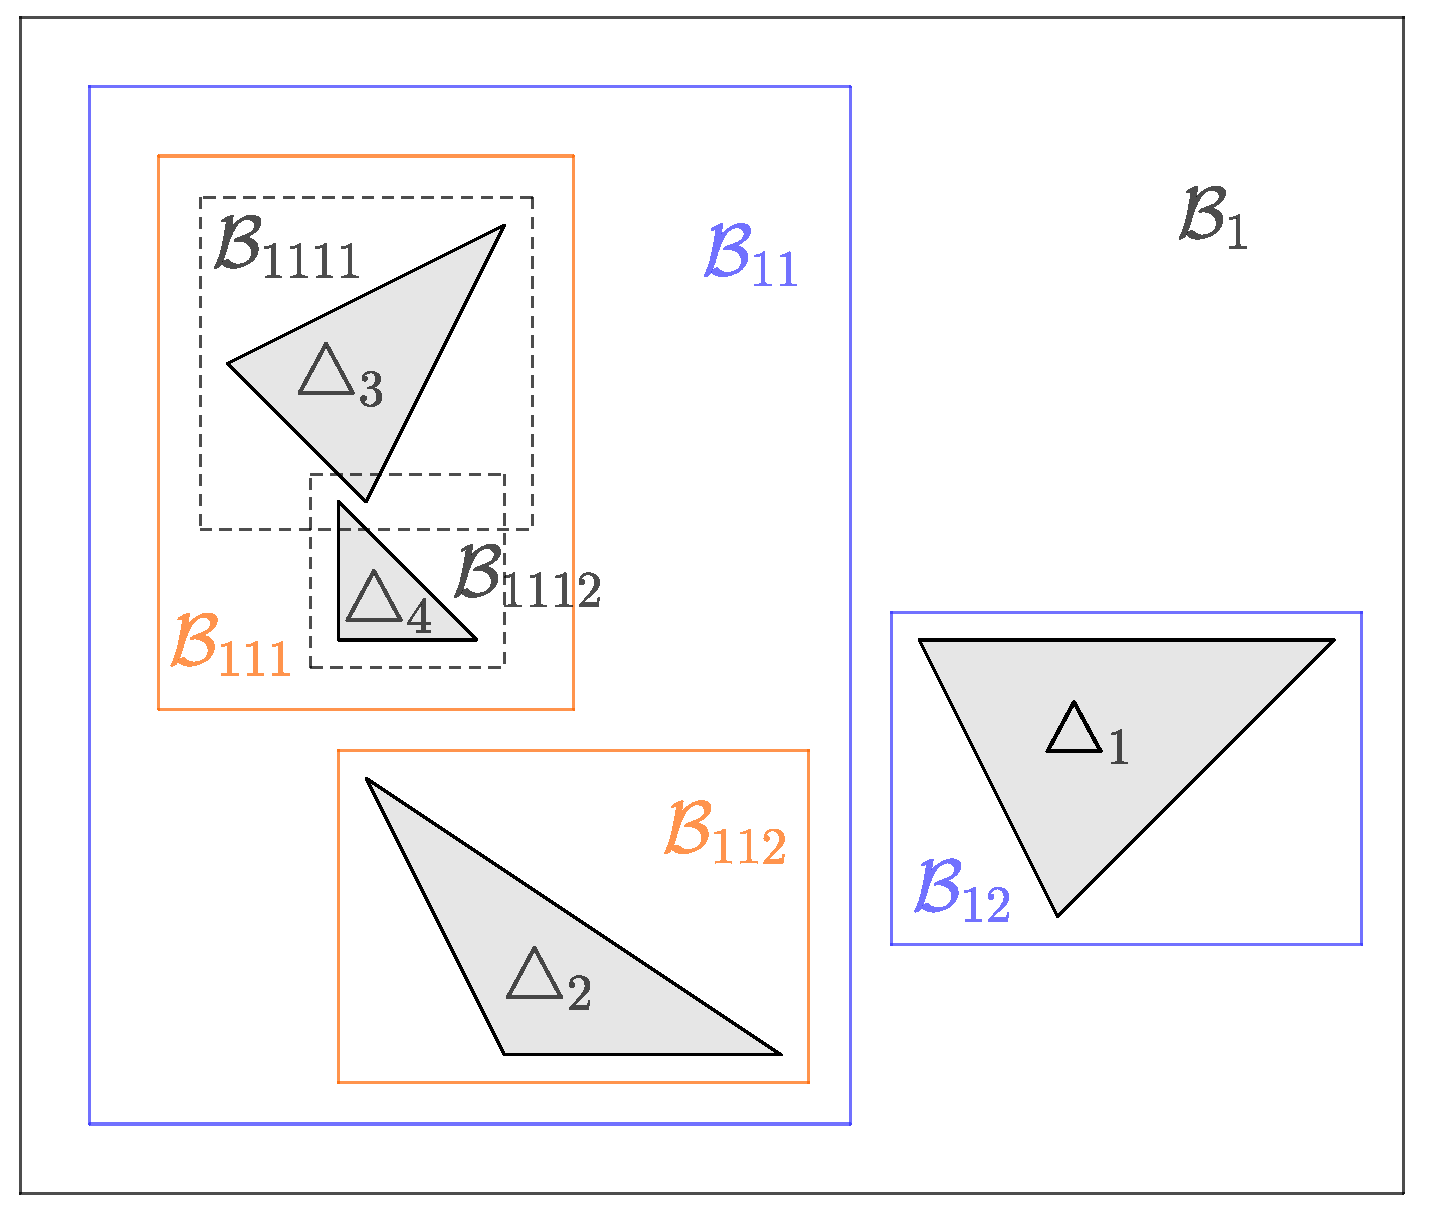
\includegraphics[width=0.95\textwidth]{images/bvh_bounding_boxes.pdf}
        \end{subfigure}
        \begin{subfigure}[b]{0.49\textwidth}
          \center
          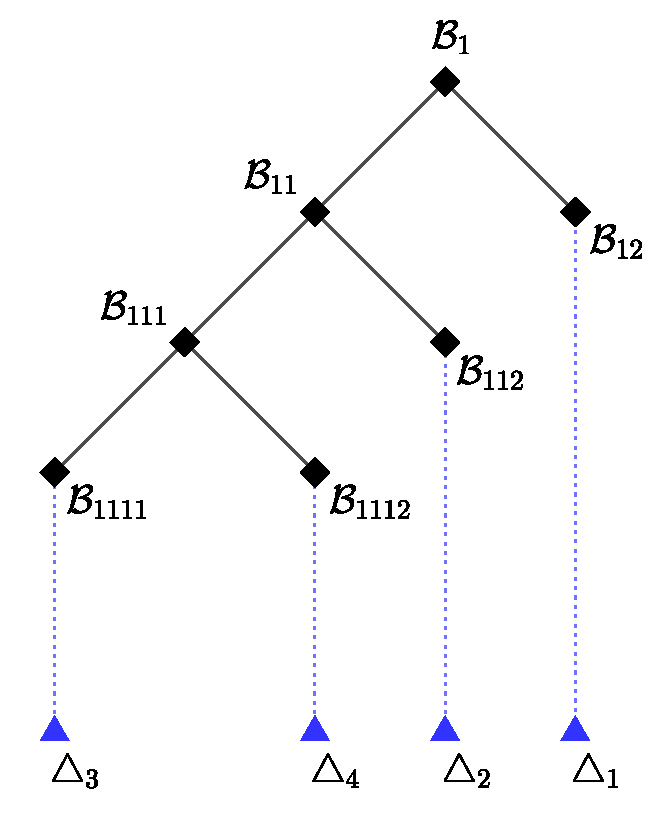
\includegraphics[width=0.75\textwidth]{images/bvh_tree.pdf}
        \end{subfigure}
        \caption{%
          Die Abbildungen zeigen die skizzenhafte Darstellung einer möglichen BVH einer Szene bestehend aus den Dreiecken $\triangle_1$, $\triangle_2$, $\triangle_3$ und $\triangle_4$.
          Im linken Bild sind die \textit{Bounding Boxes} der BVH und im rechten Bild deren zugehörige Verknüpfungen im Sinne eines Baums gezeigt.
        }
      \end{figure}
    % subsection linear_bounding_volume_hierarchies (end)

    \subsection{Path Tracing} % (fold)
    \label{sub:path_tracing}
      \subsubsection{Quasi-Monte-Carlo-Methoden} % (fold)
      \label{ssub:monte_carlo_methoden}

      % subsubsection monte_carlo_methoden (end)

      \subsubsection{Light Caching} % (fold)
      \label{ssub:light_caching}

      % subsubsection light_caching (end)

      \subsubsection{Reflexions- und Brechungsmodelle} % (fold)
      \label{ssub:reflexions_und_brechungsmodelle}

      % subsubsection reflexions_und_brechungsmodelle (end)
    % subsection path_tracing (end)

    \subsection{Optimierungen auf CPU} % (fold)
    \label{sub:optimierungen_auf_cpu}
      \subsubsection{Threadpools, OpenMP, mctp} % (fold)
      \label{ssub:threadpools}

      % subsubsection threadpools (end)

      \subsubsection{SIMD intrinsics} % (fold)
      \label{ssub:simd_intrinsics}

      % subsubsection simd_intrinsics (end)
    % subsection optimierungen_auf_cpu (end)

    \subsection{Übertragung auf die GPU} % (fold)
    \label{sub:uebertragung_auf_die_gpu}
      Funktionsweise GPU, textures, CUDA, SIMD
    % subsection übertragung_auf_die_gpu (end)
  % section beschleunigungsstrukturen_optimierung_und_weitere_features (end)
\end{document}